\documentclass{article}
\usepackage[preprint]{neurips_2026}
\usepackage[utf8]{inputenc}
\usepackage[T1]{fontenc}
\usepackage{amsmath,amssymb,booktabs,graphicx,microtype}
\usepackage{tikz}
\usetikzlibrary{arrows.meta,positioning,fit}
\usepackage[colorlinks=true,citecolor=blue,linkcolor=blue,urlcolor=blue]{hyperref}
\urlstyle{same}
\title{Learning-Oriented Global Experience Selection\\for Small Language Agents}
\author{Anonymous Authors}
\begin{document}
\maketitle
\begin{abstract}
Experience that is easy for an agent to imitate need not be the most useful material for improving its behavior. We study learning-oriented experience selection for a 4B language agent, making the admissible selection space explicit. A complete factorial development study compares nine selectors across two fixed historical experience pools, eight initialization seeds, and two sampling seeds. It trains 288 students and evaluates them with a common executor on 128 fresh development task groups. Under equal global selection freedom, 256 distinct contents, and 768 training presentations, optimizer-aware gradient selection attains 81.45\% and 73.19\% success in the two pools. It exceeds global random selection by 8.25 and 5.96 percentage points, and global high-NLL selection by 4.10 and 4.05 points. All eight initialization-level contrasts are positive in both pools against both global baselines. Allowing global selection helps the gradient rule but hurts the random rule, exposing an interaction between the ranking criterion and the coverage constraint. We retain matched-coverage comparisons, complete training curves, source differences, actual token costs, and limits of length-controlled interpretation. A separately frozen replication on 128 reserved task groups is running; this version reports no partial replication outcomes.
\end{abstract}

\section{Introduction}
Agent harnesses improve task completion through examples, feedback, memory, tools, and additional inference. Training on the resulting experience introduces a different decision: which contents should consume a limited optimization budget? Immediate collection success, action predictability, and post-training behavior are distinct quantities. A successful action can be redundant, while an unfamiliar action can be useful or simply difficult to learn.

This paper focuses on the selected training corpus and the resulting student. We start from two existing experience pools rather than attributing all subsequent differences to their collectors. The student, training recipe, public-example executor, and evaluation task panel are fixed. We vary the selection criterion and whether selection must preserve a reference task/action schedule. This makes it possible to assess both the practical effect of a complete selector and the interpretation supported by a coverage-controlled intervention.

The final comparison retains an important distinction. A global gradient selector should be compared with baselines that can also change coverage. Beating a coverage-constrained random selector alone would leave that practical comparison incomplete. We therefore add global random and global high-NLL selection under the same support and presentation budget. These additional baselines preserve the gradient selector's advantage in both pools.

Our contribution is the complete learning-oriented selection comparison, its explicit selection-space controls, and the resulting evidence about selector behavior. We instantiate optimizer-aware scoring using existing influence-based selection ideas, including LESS~\citep{xia2024less}; we do not claim the general gradient-scoring construction as new. We distinguish the observed gain of the full selection procedure from a uniquely identified gradient mechanism or a population-general data-value estimator.

\begin{figure*}[t]
\centering
\resizebox{\textwidth}{!}{%
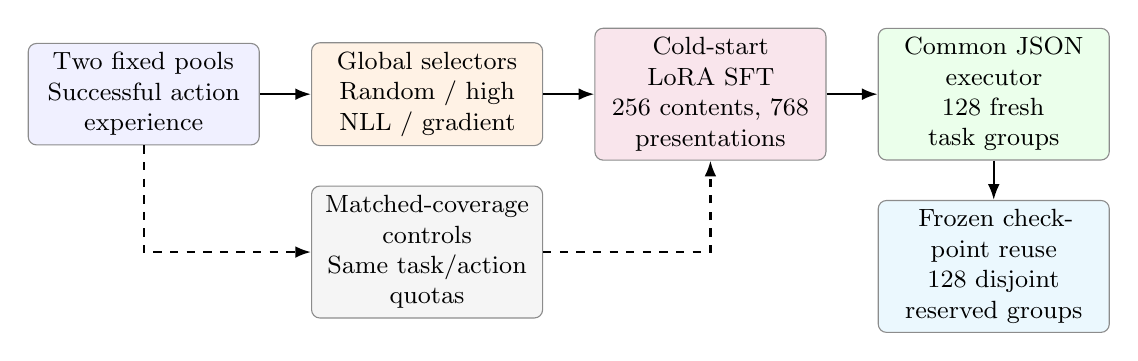
\begin{tikzpicture}[font=\small,box/.style={draw=black!45,rounded corners=3pt,align=center,minimum height=1.0cm,text width=2.7cm},arrow/.style={-{Latex[length=2mm]},thick},node distance=0.65cm]
\node[box,fill=blue!6] (pool) {Two fixed pools\\Successful action experience};
\node[box,fill=orange!10,right=of pool] (score) {Global selectors\\Random / high NLL / gradient};
\node[box,fill=purple!10,right=of score] (sft) {Cold-start LoRA SFT\\256 contents, 768 presentations};
\node[box,fill=green!8,right=of sft] (eval) {Common JSON executor\\128 fresh task groups};
\draw[arrow] (pool)--(score);\draw[arrow] (score)--(sft);\draw[arrow] (sft)--(eval);
\node[box,fill=gray!8,below=0.5cm of score] (control) {Matched-coverage controls\\Same task/action quotas};
\draw[arrow,dashed] (pool.south) |- (control.west);\draw[arrow,dashed] (control.east) -| (sft.south);
\node[box,fill=cyan!8,below=0.5cm of eval] (confirm) {Frozen checkpoint reuse\\128 disjoint reserved groups};
\draw[arrow] (eval)--(confirm);
\end{tikzpicture}}
\caption{\textbf{Experimental architecture.} Global selectors have identical admissible coverage freedom; matched controls answer a different, more constrained question. The reserved-panel replication reuses trained checkpoints. Historical collection and gradient-feature preparation costs are accounted for separately.}
\label{fig:architecture}
\end{figure*}

\section{Problem and Selection Procedure}
Let $D_s$ be a fixed historical pool, $S_p(D_s;j)$ the schedule produced by rule $p$ with sampling seed $j$, and $A_B$ the common training procedure at presentation budget $B$. Initialization/dropout seed $i$ determines the training starting state and dropout stream:
\begin{equation}
\theta_{s,p,i,j}=A_B\bigl(\theta_i,S_p(D_s;j)\bigr).
\end{equation}
With the common deployment harness $H$ and fixed panel $Q$, the behavioral endpoint is
\begin{equation}
R_{s,p,i,j}=\frac{1}{|Q|}\sum_{q\in Q}\mathbf{1}\{\operatorname{success}(\theta_{s,p,i,j},q,H)\}.
\end{equation}
The two task families have equal panel size. For two selection rules, we report
\begin{equation}
\Delta_s(p,p')=\frac{1}{IJ}\sum_{i=1}^{I}\sum_{j=1}^{J}(R_{s,p,i,j}-R_{s,p',i,j}).
\end{equation}
Each initialization first averages its two sampling replicates. Source-specific results are primary descriptions of the two fixed pools; their equal-source average is also reported. Reusing task groups across model evaluations does not create additional task identities, and 16 sampling blocks are not 16 independent initializations.

\paragraph{Likelihood baselines.} Low, middle, and high NLL use canonical action-level scores from the fixed base student. Matched selectors choose within task/action strata and preserve the reference schedule's stratum at every position and its distinct-content quotas. Global high NLL instead ranks all distinct contents without those quotas. Global random samples 256 distinct contents uniformly without replacement; repeated original rows do not increase selection probability.

\paragraph{Optimizer-aware score.} At warmup checkpoint $c$, let $g_c(e)$ be a candidate's LoRA gradient, with frozen Adam moments $m_c,v_c$. The feature follows the LESS-style expression
\begin{equation}
a_c(e)=\frac{\beta_1 m_c+(1-\beta_1)g_c(e)}{\sqrt{\beta_2 v_c+(1-\beta_2)g_c(e)^2+\epsilon}}.
\end{equation}
This frozen-state feature is not a claim of reproducing the exact bias-corrected AdamW parameter update. Let $u(x)=x/\|x\|_2$ and $b_{c,f}$ be the mean of individually normalized public-support gradients for family $f$. The implemented score is
\begin{equation}
s(e)=\max_f\sum_{c\in\{8,16,24,32\}}\tfrac14\,u(a_c(e))^\top b_{c,f}.
\end{equation}
Checkpoint averaging precedes the maximum over support families. The 40 fixed public actions contain 18 placement and 22 cleaning actions; no query answers are used. Features are evaluated in a numerically checked FP32 procedure. Final students start again from the original base, not the feature-warmup weights.

\paragraph{Common replay.} Each global rule selects 256 distinct message contents. Each set is replayed in three shuffled passes using the same schedule-generation procedure, yielding 768 presentations. The selected contents and their task/action distribution can differ. Fixed presentations and optimizer updates do not establish equal token counts or FLOPs.

\section{Experimental Design}
\paragraph{Environment and data.} We use ALFWorld's text interface~\citep{shridhar2021alfworld}, not visual robot control. The API and Generic pools contain 721 and 732 eligible action demonstrations, with 418 and 508 distinct message contents, from 35 and 29 collection tasks. These are two fixed historical sources in one environment, not randomized harness treatments or independent environments. All current studies reuse the pools and make zero new teacher calls.

\paragraph{Student and training.} Qwen3-4B-Instruct-2507~\citep{yang2025qwen3} is pinned to revision \texttt{cdbee75f17c01a7cc42f958dc650907174af0554}. LoRA~\citep{hu2022lora} uses rank 16, alpha 32, dropout 0.05, and $q/k/v/o$ attention projections. Every student receives 192 optimizer updates and 768 presentations, with global batch size four, learning rate $10^{-4}$, 0.05 warmup ratio, zero weight decay, and maximum sequence length 2,048. Initial parameter hashes match across paired selection rules. Actual input and target token totals are audited.

\paragraph{Shared executor.} Evaluation uses the same JSON action interface and two fixed public examples, task-local history length 12, environment seed 11, temperature zero, batch size eight, at most 40 calls per episode, and at most 128 generated tokens per call. There is no teacher card, retry, or cross-task memory. The inherited adapter interface combines each student's A adapter with an immutable zero-B branch; B is not updated and weights are not merged in BF16.

\paragraph{Complete matrices.} The original seven-rule development matrix trains 224 students across two sources, eight initialization seeds, and two sampling seeds. The missing global random/high-NLL baselines add 64 students. Their comparison reuses 32 existing global-gradient students and the untrained base. All models use the same 128 fresh development groups, balanced between placement and cleaning. Groups are disjoint from training, interface-calibration, and reserved replication groups. They are train-derived task groups, not official seen/unseen benchmark tests.

\paragraph{Reporting and integrity.} We report completed matrices, every initialization, negative outcomes, and descriptive dispersion. Independent audits reconstruct 97 model endpoints from raw episodes, events, request accounting, training metadata, and weight identities for the global comparison. The 564 supplementary frozen inputs and all 509 parent inputs remain unchanged. Three cloud aggregate files and 64 added native-training summaries match local records. These checks establish provenance, not statistical significance. Development comparisons remain development evidence even when they show consistent signs.

\section{Results}
\begin{table}[t]
\centering\small
\caption{\textbf{Complete development results.} Success is a percentage. Each source/rule mean averages eight initializations and two sampling seeds. Global rules have equal selection freedom. Matched rules share task/action quotas. The same-panel base is 67.188\%.}
\label{tab:main}
\begin{tabular}{llrr}\toprule
Space & Rule & API & Generic\\\midrule
Matched & Random & 77.344 & 68.652\\
& Low NLL & 72.070 & 67.627\\
& Middle NLL & 73.975 & 68.750\\
& High NLL & 78.906 & 68.408\\
& Gradient high & 77.295 & 71.875\\
& Gradient low & 72.559 & 65.186\\\midrule
Global & Random & 73.193 & 67.236\\
& High NLL & 77.344 & 69.141\\
& Gradient & \textbf{81.445} & \textbf{73.193}\\\bottomrule
\end{tabular}
\end{table}

\subsection{Equal Global Selection Freedom}
Global gradient selection reaches 81.445\% in API and 73.193\% in Generic (Table~\ref{tab:main}). Its differences from global random are +8.252 and +5.957 percentage points; its differences from global high NLL are +4.102 and +4.053 points. All eight initialization-level mean differences are positive in each source against each global comparator. These are paired descriptive outcomes, not calibrated population confidence statements.

\begin{figure*}[t]\centering
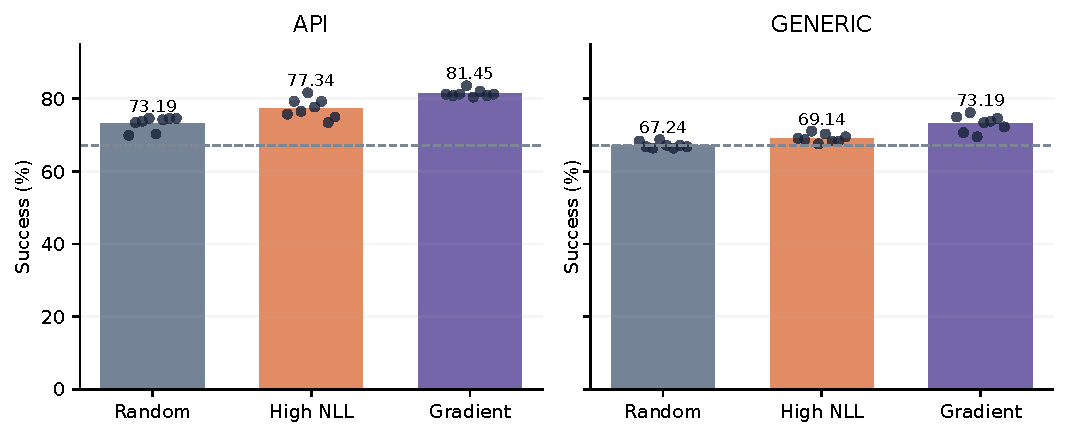
\includegraphics[width=0.88\textwidth]{figures/global-main.pdf}
\caption{\textbf{Global comparison on fresh development groups.} Each dot is an initialization's mean over two sampling seeds. Bars average eight initializations; the dashed line is the same-panel untrained base. The global baselines share support size and replay budget with the gradient rule.}
\label{fig:global}
\end{figure*}

The additional comparison matters: the previously available random comparator was coverage matched. Its disadvantage could not by itself establish the global rule's benefit over an equally unconstrained alternative. The two added baselines close that comparison gap; the observed global-gradient advantage remains in both fixed pools.

\subsection{Selection Criterion Interacts with Coverage Constraints}
Moving from matched to global selection changes Random by $-4.150$ points in API and $-1.416$ in Generic. The gradient rule changes by $+4.150$ and $+1.318$ points. High NLL changes by $-1.562$ and $+0.732$ points. Selection freedom is therefore not uniformly beneficial: its association with student performance depends on the ranking rule (Figure~\ref{fig:interaction}).

These changes also alter selected contents, frequencies, and histories. We do not interpret their difference as a pure causal mediation fraction for coverage, or assert that action entropy alone explains the result. The matched and global conditions characterize different admissible interventions.

\begin{figure*}[t]\centering
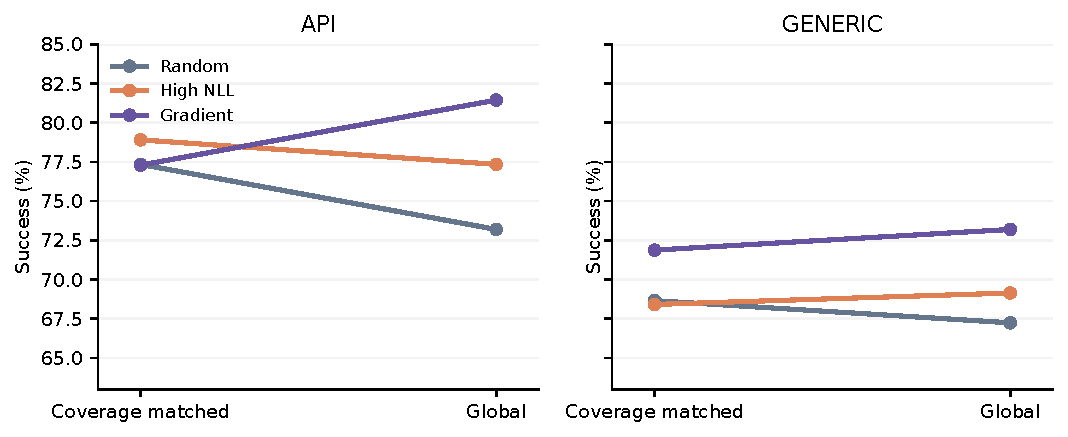
\includegraphics[width=0.88\textwidth]{figures/selection-coverage-interaction.pdf}
\caption{\textbf{Selection rule $\times$ admissible coverage.} The common student and presentation budget are fixed. Relaxing the task/action quotas helps the gradient selector and hurts Random in both pools. Lines connect complete experimental means, not intermediate learning checkpoints.}
\label{fig:interaction}
\end{figure*}

\subsection{Initialization-Level Consistency}
Figure~\ref{fig:seeds} retains every initialization-level contrast. Differences from global random range from 6.250 to 11.328 points in API and 0.781 to 9.766 in Generic. Differences from global high NLL range from 1.562 to 7.422 in API and 1.953 to 6.250 in Generic. Positive signs are not confined to one favorable seed or one source. The eight initializations each average two sampling replicates; their 16 component blocks are not treated as independent initialization draws.

\begin{figure*}[t]\centering
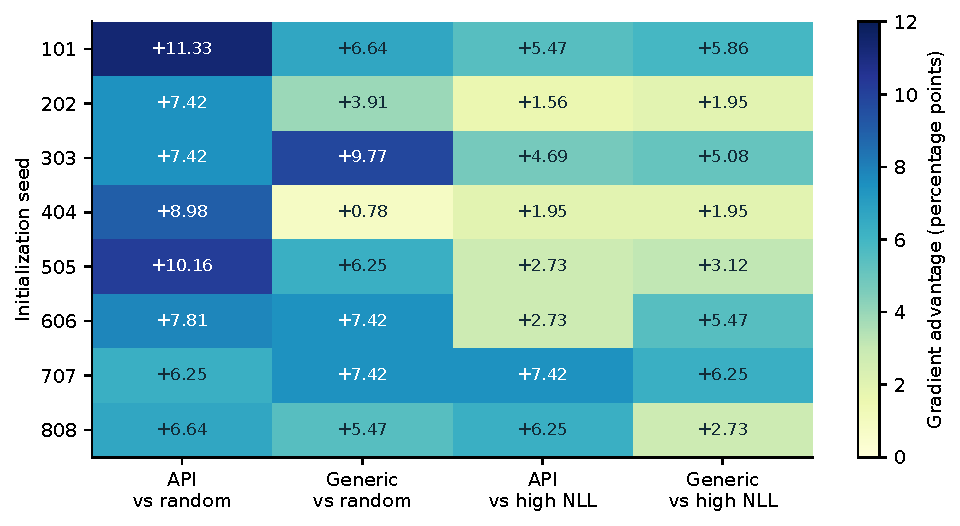
\includegraphics[width=0.78\textwidth]{figures/paired-initializations.pdf}
\caption{\textbf{Every paired initialization.} Cells show gradient minus comparator success, in percentage points, after averaging the two sampling seeds. All values are retained. There are no significance stars or confidence-interval interpretations.}
\label{fig:seeds}
\end{figure*}

\subsection{Likelihood and Behavioral Utility}
Low, middle, and high NLL obtain 72.070\%, 73.975\%, and 78.906\% in the API matched conditions; the Generic ordering is smaller and nonmonotonic. The lowest imitation NLL is not the best downstream choice. Conversely, high NLL is a useful strong baseline, and its matched API result exceeds matched gradient high. The global result does not erase this source- and constraint-dependent ordering.

The corpus-level scatter in Appendix~\ref{app:scatter} includes all 36 fixed source/rule/sampling schedules. Each point averages eight trained initializations. Schedules overlap and are not 36 independent corpora; the plot is descriptive, without a fitted significance claim.

\section{Frozen Reserved-Task Replication}
A new protocol is frozen before the first reserved-task model call. It reuses all 96 global-rule checkpoints plus the untrained base on 128 disjoint reserved task groups (12,416 episodes), with no additional training. Both sources, all eight initializations, and both sampling seeds remain fixed. The primary analysis is a finite-panel descriptive paired replication: endpoint means, initialization-level differences and SD, and development/replication comparisons. No uncalibrated population p-value, confidence interval, or equivalence claim is planned. This explicitly replaces the earlier draft's prospective population-inference proposal; the choice is fixed before replication outcomes.

\textbf{Status of this version: evaluation is running. No partial reserved-task outcome is included.} Official seen/unseen benchmark tests are not used. The completed protocol and all resulting endpoints will be reported regardless of direction.


\section{Costs and Limitations}
\paragraph{Measured cost.} The 224-student development study consumes 62.146 cumulative GPU-hours including its stated preparation costs. The 64 added global baselines consume 17.419 hours; the global comparison itself reuses existing gradient students and the base. The final replication reuses all 97 checkpoints and has a 30.5-hour cap, so supplementary baselines plus replication remain under the 48 additional GPU-hour finishing budget. Prior source collection and historical experiments remain separately accounted costs.

\paragraph{Support and token budgets.} Gradient scoring uses 40 public target-family actions and its feature-warmup cost; those actions are not added to student SFT. The same public examples are available to the deployment executor, but selector computations differ. Equal presentations do not imply equal FLOPs: API matched gradient-high inputs average 476,314 tokens versus 500,016 for gradient-low; Generic averages 510,404 versus 527,626. We report this difference rather than labeling the schedules strictly compute matched.

\paragraph{Limits of mechanism isolation.} A CPU-only strict length-matching check fixes task/action budgets and target-token length while checking input bins of 0, 8, 16, and 32 tokens. It requires at most 1\% input-token imbalance and retention of at least 25\% of the original high/low gradient-score gap in every source/sampling condition. No width passes. At width 32, API retains 3.45--5.23\% of the gap and Generic 17.06--18.17\%. This identifies insufficient conditional choice for that proposed control, not evidence that length explains the downstream gain. We do not claim a length-independent gradient mechanism.

\paragraph{Scope.} The results concern one backbone, one text environment, two fixed pools, and finite task panels. They are not robot/VLA results, multi-round continual-learning results, or a second-environment learning replication. Historical WebShop runs are interface calibration only. Existing gradient-selection literature must receive attribution; a higher endpoint does not establish algorithmic priority. The official benchmark seen/unseen sets remain unused.

\section{Conclusion}
Global learning-oriented selection produces a higher-performing student than both equally global random and high-NLL selection in the completed development study. The ranking criterion and admissible coverage constraint interact, and the full comparator set prevents practical gain from being confused with coverage-controlled attribution. We retain source differences, simple strong baselines, individual initializations, and limitations on length and generalization. Reserved-task results will be incorporated only after the frozen full matrix completes.

\begingroup\footnotesize\setlength{\bibsep}{2pt}
\bibliographystyle{plainnat}
\bibliography{references}
\endgroup

\clearpage\appendix
\section{Recorded Training Dynamics}
\begin{figure*}[h]\centering
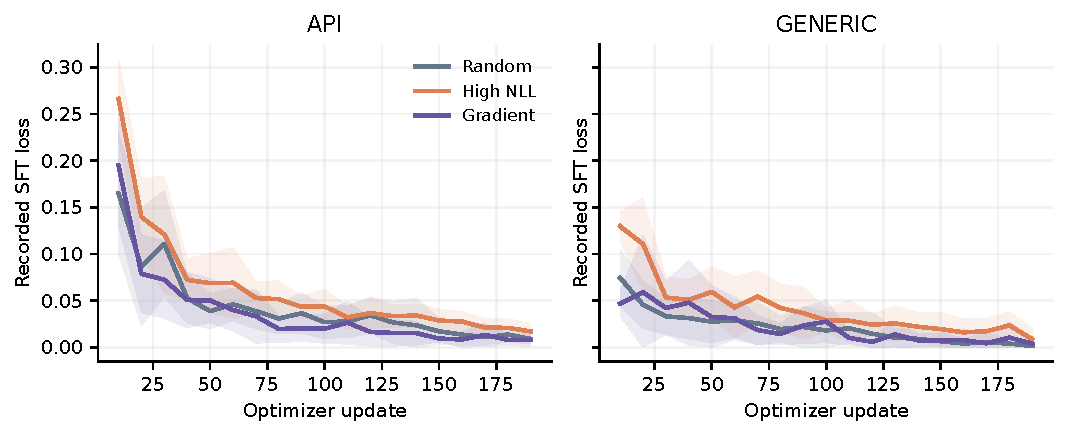
\includegraphics[width=0.9\textwidth]{figures/training-loss.pdf}
\caption{Actual Trainer loss at logging steps 10 through 190. Each line averages 16 model histories per source/rule; shading is their descriptive SD, not a confidence interval. These are training-loss curves, not task-success learning curves. No value is fabricated for an unlogged update.}
\end{figure*}
The curves help audit optimization and show that low training loss alone is insufficient to rank behavioral utility. Their bands retain training variation. All students still run the fixed 192 updates; the final two updates do not create a new recorded loss point.

\section{Aggregate Action Composition}
\begin{figure*}[h]\centering
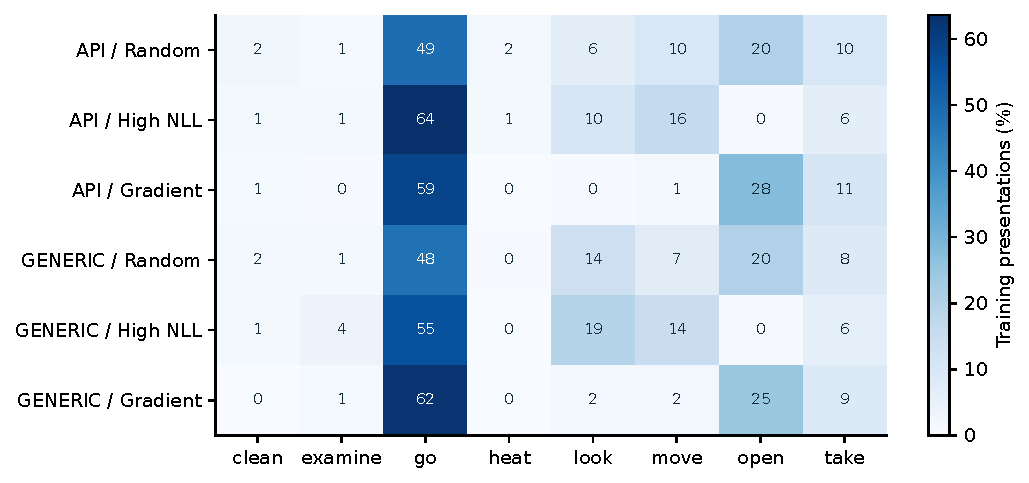
\includegraphics[width=0.92\textwidth]{figures/action-coverage.pdf}
\caption{Action-family composition of the selected 768-presentation schedules, averaged over the two sampling seeds. Values are percentages. Only aggregate action categories are shown, with no task identities. Different distributions are observed properties of the selectors, not an identified causal explanation.}
\end{figure*}
Global selection is allowed to choose these distributions; matched comparisons fix the reference task/action position and distinct-content quotas. The distinction is why both comparisons are retained rather than treating one as a replacement for the other.

\section{Imitation-Likelihood Scatter}\label{app:scatter}
\begin{figure*}[h]\centering
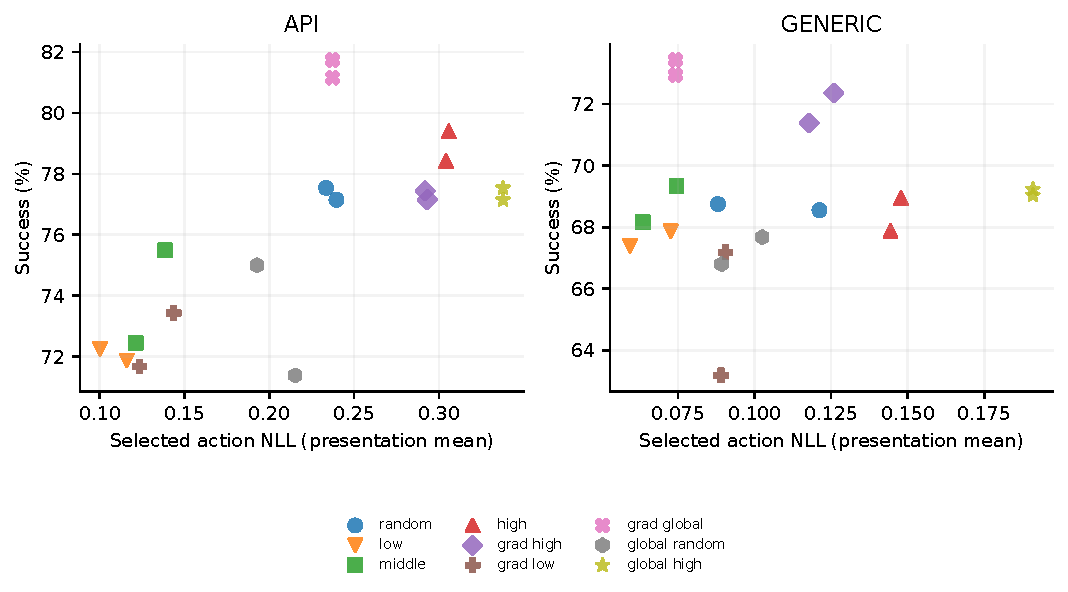
\includegraphics[width=0.96\textwidth]{figures/imitation-learning.pdf}
\caption{All 36 source/rule/sampling schedules. Horizontal coordinates are mean selected action NLL weighted by training presentations; vertical coordinates average the eight actual student initializations. Overlapping schedules are not independent corpus samples. No regression significance or new utility predictor is inferred from this plot.}
\end{figure*}

\section{Retained Historical Evidence}
Earlier complete-pass scheduling improves success over subset replay by 5.176 and 1.270 points at the same update/presentation budget. Task-matched low-NLL selection is below Random by 17.773 and 7.812 points; task/action matching reduces the descriptive gap to 4.818 and 2.995 points. The separate canonical-scoring retraining comparison gives low-NLL-minus-Random differences of $-3.516$ and $-3.060$ points. These studies use older, repeatedly examined development panels and remain separate evidence, rather than being pooled into the fresh-panel estimate.

The original teacher-assisted versus ReAct source comparison also remains: its common-success matched adaptation-AUC difference is $-3.56$ points across three seeds. Within-pool selection gains do not resolve the missing full-eligible source comparison or establish that one collector produces a generally better learner.

\section{Reproducibility and Version Boundaries}
Source protocols, numerical scoring checks, training/initialization roles, final aggregates, raw-audit receipts, cloud-file hashes, and figure data are versioned separately. Raw task identities, conversations, requests, and weights stay local. The global development data bind 564 frozen inputs; the original parent binds 509. The reserved-panel run binds its own 1,025 inputs and the benchmark execution gate. Completed model files can be relocated only with byte verification and original-path links, preserving composition revisions.

This manuscript snapshot contains completed development outcomes and explicitly labeled reserved-panel status. It does not convert partial task successes into a method result. Generated confirmation tables may update only from the complete 97-model audited output, preserving the earlier snapshot.
\end{document}
